\part{Software Quality and Quality Assurance}
\frame{\partpage}

\begin{frame}{Learning Outcomes}
	In this section you will learn how to...
	
	\begin{itemize}
		\item \textbf{Explain} what `quality' is
		\item \textbf{Explain} what `quality assurance' is
		\item \textbf{Discuss} the role of quality assurance in software engineering
	\end{itemize}
\end{frame}

\begin{frame}{Further Reading}
	\begin{itemize}
		\item Pressman, R.S. (2009) \textit{Software Engineering: A Practitioner's Approach}. 7th Edition. McGraw-Hill.
		\item Kaner, C., Falk, J. And Nguyen, H.Q. (1999) \textit{Testing Computer Software}. John Wiley and Sons.
	\end{itemize}
\end{frame}

\begin{frame}{Software Quality}
    ``Bad software plagues nearly every organisation that uses computers, causing lost work hours during computer downtime
    lost or corrupted data, missed sales opportunities, high IT support, and maintenance costs, and low customer satisfaction''
    \vspace{2ex}
    (ComputerWorld, 2005)
\end{frame}

\begin{frame}{Software Quality}
    ``The Sorry State of Software Quality---quality has gotten worse!''
    \vspace{2ex}
    (InfoWorld, 2006)
\end{frame}

\begin{frame}{Software Quality}
	So, what does quality look like in games? \pause
	
	\begin{itemize}
		\item ``A characteristic or attribute of something.'' \pause
		\item Quality may relate to several aspects of games: \pause
		\begin{itemize}
			\item \textbf{the quality of the design}: the aesthetic is specified to accurately meet the desires and 
			pleasures of the target audience; provides a distinctive experience; etc. \pause
			\item \textbf{the quality of the implementation}: the game mechanics are able to achieve the intended
			aesthetic; the game is well-implemented...
		\end{itemize}
	\end{itemize}
\end{frame}

\begin{frame}{Software Quality}
	\begin{center}
        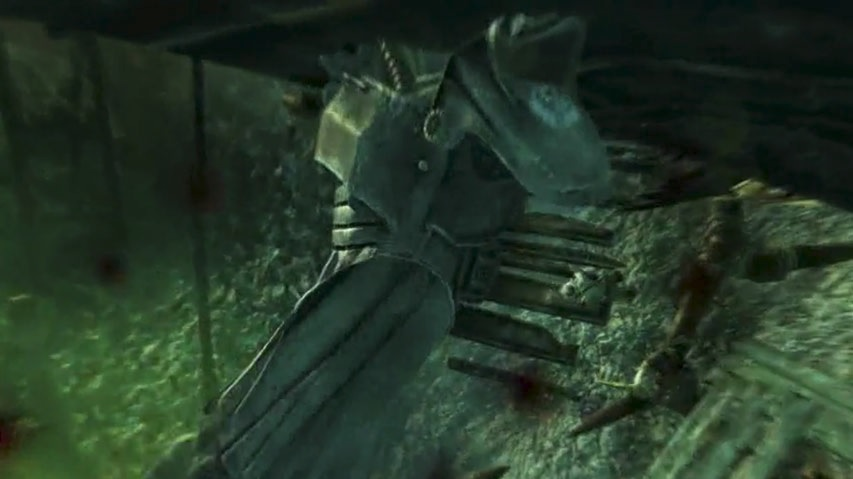
\includegraphics[width=\textwidth]{fallout3_collision_bugs.jpg}
    \end{center}
\end{frame}

\begin{frame}{Software Quality}
	\begin{center}
        
\includegraphics[width=\textwidth]{ac_graphics_bug.jpg}
    \end{center}
\end{frame}

\begin{frame}{Software Quality}
	%\movie[width=3cm,height=2cm,poster]{}{bird_boost.avi}
	\begin{center}
        \url{https://www.youtube.com/watch?v=VhenntkfAgU}
    \end{center}
\end{frame}

\begin{frame}{Software Quality}
	Today, software quality in games remains an issue, but who is to blame? \pause
	
	\begin{itemize}
		\item Players blame developers, arguing that sloppy practices lead to low-quality software. \pause
		\item Investors blame developers for not understanding what players want and what is `good enough' to maximise profit. \pause
		\item Developers blame the design team and their publisher, arguing that irrational delivery dates and continuous
		change force them to deliver software before it can be adequately tested.
	\end{itemize}
\end{frame}

\begin{frame}{Socrative \texttt{6E8NSW3IN}}
	So, who is responsible?
	\begin{itemize}
		\item In pairs.
		\item Discuss for 2-minutes whether designers, developers, or publishers are responsible for software quality.
		\item \textbf{Suggest} which parties are responsible \textbf{and justify} your answer. 
	\end{itemize}
\end{frame}

\begin{frame}{Socrative \texttt{6E8NSW3IN}}
	But wait...what exactly is quality?
	
	\begin{itemize}
		\item In pairs.
		\item Discuss for 2-minutes what `software quality' means in the context of game development.
		\item \textbf{Give} a definition for `game software quality'. 
	\end{itemize}
\end{frame}

\begin{frame}{Software Quality}
    {\small
	``Quality...you know what it is, yet you don't know what it is. But that's self-contradictory. But some things are better than 
	others, that is, they have more quality. But when you try to say what the quality is, apart from the things that have it, it all 
	goes poof! There's nothing to talk about. But if you can't say what Quality is, how do you know what it is, or how do you know 
	that it even exists? If no one knows what it is, then for all practical purposes it doesn't exist at all. But for all practical purposes 
	it really does exist. What else are the grades based on? Why else would people pay fortunes for some things and throw others
	 in the trash pile? Obviously some things are better than others...but what's the betterness?...So round and round you go, 
	 spinning mental wheels and nowhere finding anyplace to get traction. What the hell is Quality? What is it?''}
	\vspace{2ex}
	(Robert Persid, 1974)
\end{frame}

\begin{frame}{Software Quality}
	\begin{itemize}
		\item \textbf{transcendental view}: quality is something immediately recognisable, but cannot be explicitly defined. \pause
		\item \textbf{pragmatic view}: relative to utility and specific goals. If something meets our goals, it exhibits quality.  \pause
		\item \textbf{commercial view}: the specification is key. If the specification is sound and the product conforms to the
		specification, it exhibits quality. 
	\end{itemize}
\end{frame}

\begin{frame}{Software Quality}
	\begin{itemize}
		\item \textbf{product view}: quality is tied to inherent characteristics (e.g. functions and features) of a product.  \pause
		\item \textbf{value-based view}: quality is based on how much a customer is willing to pay.  \pause
		\item In practice, perception of quality tends to combine these different views in subtle and nuanced ways.
	\end{itemize}
\end{frame}

\begin{frame}{Software Quality}
	``An effective software process applied in a manner that creates a useful product that provides measurable
	value for those who produce it and those who use it.''
	\vspace{2ex}
	(Bes, 2004)
\end{frame}

\begin{frame}{Socrative \texttt{6E8NSW3IN}}
	Can we now construct a better definition of software quality in games?
	
	\begin{itemize}
		\item In pairs.
		\item Discuss for 2-minutes what `software quality' means in the context of game development.
		\item \textbf{Give} a definition for `game software quality'. 
	\end{itemize}
\end{frame}

\begin{frame}{Quality Assurance}
	\begin{itemize}
		\item An \textbf{effective development process} establishes the infrastructure that supports any effort towards high quality. \pause
		\item The management aspects create checks and balances to help avoid project chaos---a key contributor to poor quality. \pause
		\item Software engineering practices empower developers to analyse and review their product. \pause
		\item Umbrella activities, such as project management and code reviews, are key factors in determining quality and have just as an
		important role as any other specific source code quality assurance practice.
	\end{itemize}
\end{frame}

\begin{frame}{Quality Assurance}
	In order to assure quality in games, we need to know what to measure. David Garvin (1987) has some suggestions: \pause

	\begin{itemize}
		\item \textbf{performance}: does the software deliver all content, functions, and features that are specified as part of the
		 requirements model in a way that provides value to the end-user? \pause
		\item \textbf{features}: does the software provide features that surprise and delight first-time end-users? \pause
		\item \textbf{reliability}: does the software deliver all features and capability without failure? Is it available when it is needed? 
		 Does it deliver functionality that is error free?
    \end{itemize}
\end{frame}

\begin{frame}{Quality Assurance}
    \begin{itemize}
		\item \textbf{conformance}: does the software conform to local and external software standards that are relevant to the 
		application? Does it conform to de facto design and coding conventions? For example, does the user interface conform to accepted 
		design rules for menu selection or data input? \pause
		\item \textbf{durability}: Can the software be maintained (changed) or corrected (debugged) without the inadvertent generation 
		of unintended side effects? Will changes cause the error rate or reliability to degrade with time? 
    \end{itemize}
\end{frame}

\begin{frame}{Quality Assurance}
    \begin{itemize}
		\item \textbf{serviceability}: Can the software be maintained (changed) or corrected (debugged) in an acceptably short time period. 
		Can support staff acquire all information they need to make changes or correct defects? \pause
		\item \textbf{look-and-feel}: Most of us would agree that an aesthetic entity has a certain elegance, a unique flow, and an obvious 
		`presence' that are hard to quantify but evident nonetheless. \pause
		\item \textbf{socio-cultural context}: In some situations, you have a set of prejudices that will influence your perception of quality. 
	\end{itemize}
\end{frame}

\begin{frame}{Quality Assurance}
Other definitions to explore and factors to consider in your own time:

    \begin{itemize}
        \item McCall's Quality Factors
        \item ISO 9126 Quality Factors
        \item Targeted Factors
        \item IEEE 610.12 Software Assurance
    \end{itemize}
\end{frame}

\begin{frame}{Socrative \texttt{6E8NSW3IN}}
	Why are these factors important in games?
	
	\begin{itemize}
		\item In pairs.
		\item Discuss for 2-minutes why quality assurance is important to game development.
		\item \textbf{Illustrate TWO} reasons why quality assurance is important. Use examples to support your answer. 
	\end{itemize}
\end{frame}

\begin{frame}{Quality Assurance}
Why are these factors important? \pause

    \begin{itemize}
        \item If you produce a software system that has terrible quality, you lose because no one will want to buy it.  \pause
        \item If on the other hand you spend infinite time, extremely large effort, and huge sums of money to build the absolutely perfect piece of software,
         then it's going to take so long to complete and it will be so expensive to produce that you'll be out of business anyway.  \pause
        \item Either you missed the market window, or you simply exhausted all your resources. 
    \end{itemize}
\end{frame}

\begin{frame}{Quality Assurance}
    \begin{itemize}
        \item Some aim to that magical middle ground where the product is good enough not to be rejected right away, but also not the object of so much 
        perfectionism and so much work that it would take too long or cost too much to complete.  \pause
        \item So-called `good enough' software tends to deliver high quality functions and features that end-users desire, but at the same time may risk delivering
        other more obscure or specialized functions and features that contain bugs. \pause
        \item Large companies can get away with serious bugs at launch (e.g. Activision-Blizzard and Diablo 3)---but, smaller indies risk permanent damage to their reputation.
    \end{itemize}
\end{frame}

\begin{frame}{Activity}
    \begin{itemize}
        \item Organise into your COMP150 groups
        \item Read \url{http://blog.codinghorror.com/code-smells/}
        \item As a group, identify \textbf{three} code smells that are present in your COMP150 game code
        \item Discuss how you might go about refactoring to remove the smells
    \end{itemize}
\end{frame}

